\documentclass[fr]{../../../../../../eplexam}

\usepackage{enumitem}

\newcommand{\hsp}{\hspace{5mm}}
\newcommand{\tx}{\hsp \textup}
\setlist[itemize]{label=\textbullet}
\renewcommand{\r}{\textbf{r}}
\renewcommand{\k}{\textbf{k}}

\hypertitle{Mécanique des sols}{6}{GCIV}{1072}{2018}{Juin}{Majeure}
{Théo Gladsteen}
{Benoît Pardoen}

%Vu que le travail pour ma partie portait essentiellement sur les 3 premiers chapitres du cours, l'examen portera exclusivement sur le chapitre 4 "Les électrons dans le cristal" (il y a deux fichiers PDF sur Moodle dont des notes manuscrites très complètes).

%Je pourrai demander des définitions, des concepts généraux, des comparaisons entre différentes approximations ou vous proposer un exercice (voir notamment les exercices 5 et 6 sur Moodle). Je ne demanderai pas de restituer une démonstration.

\section{Exercices}
\subsection{Question 1 (4 points)}
On prélève dans de l'argile des échantillons sur lesquels on effectue 3 essais (CU + u).

\begin{center}
\begin{tabular}{ccc}
\textbf{Contrainte} & \textbf{Contrainte} & \textbf{Pression interstitielle}\\
\textbf{latérale} & \textbf{verticale} & \textbf{à la rupture}\\
$\mathbf{\sigma_3\,[kPa]}$ & $\mathbf{\sigma_1\,[kPa]}$ & $\mathbf{u\,[kPa]}$\\
\hline
100 & 321 & 40\\
150 & 408 & 71\\
200 & 494 & 102\\
\end{tabular}
\end{center}

Déterminer $\phi'$ et $c'$ via \textbf{deux manières différentes}.




\begin{minipage}{0.7\linewidth}
\subsection{Question 2 (4 points)}
On considère la fondation rectangulaire suivante qui représente une charge répartie $q = 55\,kPa$ :
\begin{enumerate}
\item A partir de l'abaque adéquat, déterminer la contrainte au point A pour des profondeurs de $z=0m$, $z=2m$ et $z=4m$
\item En utilisant le principe de superposition, trouver les contraintes en B, C et D pour $z=4m$
\end{enumerate}
\end{minipage}
\begin{minipage}{0.3\linewidth}
\begin{center}
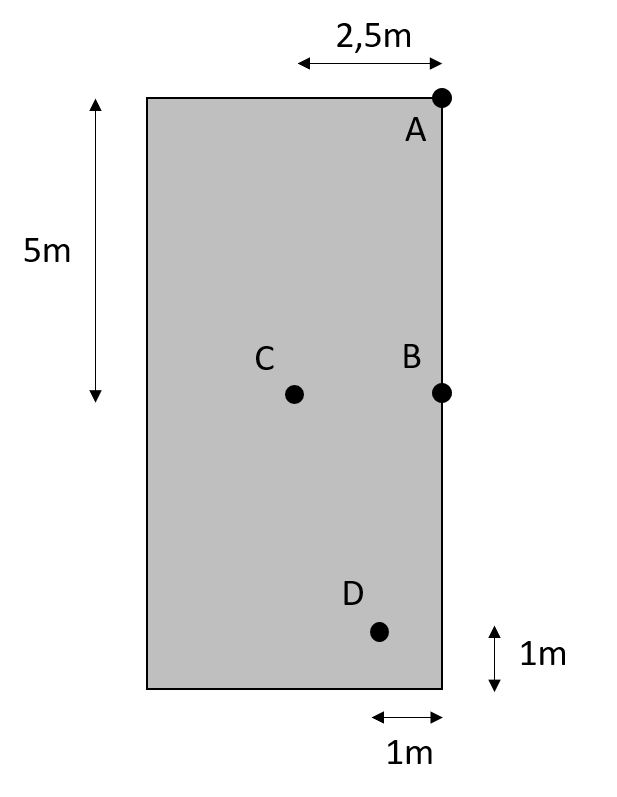
\includegraphics[width=0.8\linewidth]{ex2}
\end{center}
\end{minipage}




\newpage
\subsection{Question 3 (6 points)}
On considère le massif suivant :

\begin{center}
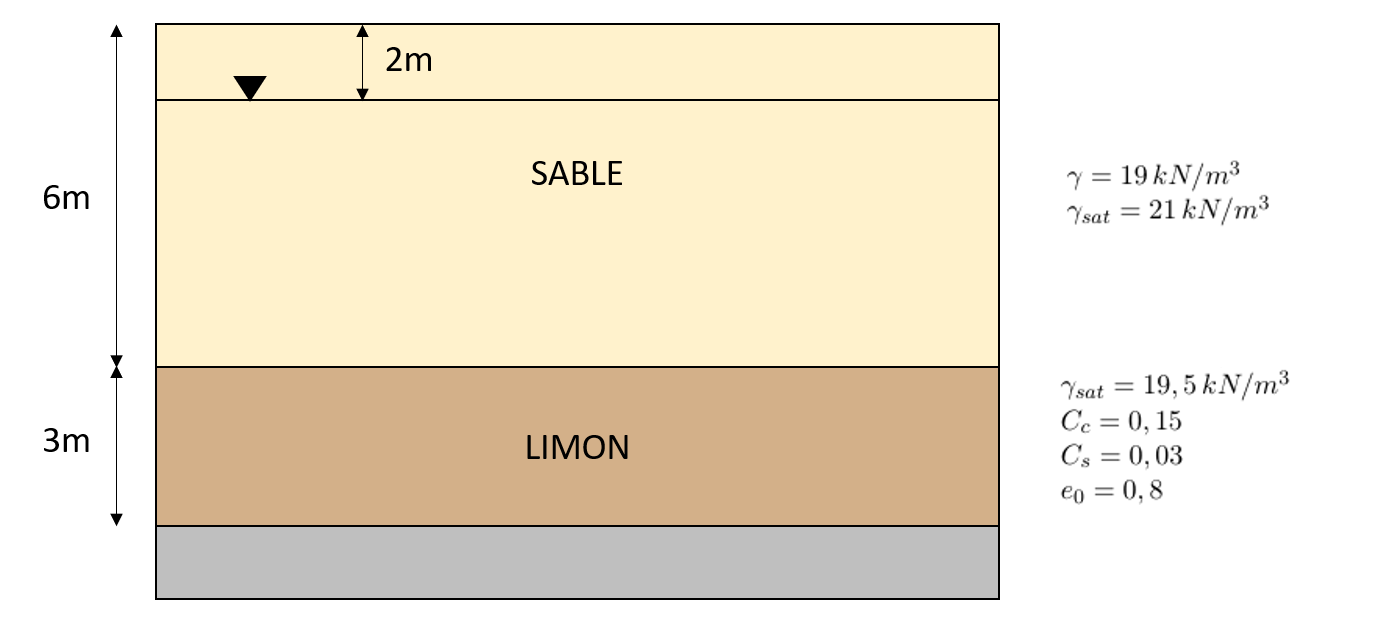
\includegraphics[width=0.7\linewidth]{ex1}
\end{center}


\begin{itemize}
\item \textbf{Phase 1 :} Rabattement de la nappe de 3m par rapport à sa position initiale.
\item \textbf{Phase 2 :} Création d'une fouille de 4m de profondeur.
\item \textbf{Phase 3 :} Construction d'un radier et de caves qui ajoutes 100kPa
\item \textbf{Phase 4:} Relâchement de la nappe.
\item \textbf{Phase 5:} Construction d'un immeuble qui rajoute 200kPa.
\end{itemize}

On considère que les distributions sont uniformes dans les couches et que le temps entre chaque phase est assez long pour que l'on atteigne la fin de la consolidation de chaque phase.\\

Sachant que la contrainte initiale (phase 0) de la couche de limon correspond à la contrainte de préconsolidation, on demande de :

\begin{enumerate}
\item Évaluer le tassement moyen du limon et son indice des vides pour chaque phase
\item Dessiner le diagramme $e-\log \sigma'_v$ (quadrillage logarithmique donné)
\end{enumerate}
%$\gamma = 19\,kN/m^3$\\
%$\gamma_{sat} = 21\,kN/m^3$\\
%$\gamma_{sat} = 19,5\,kN/m^3$\\
%$C_c = 0,15$\\
%$C_s=0,03$\\
%$e_0 = 0,8$\\













\newpage
\subsection{Exercice 4 (6 points)}
Soit le mur de soutènement suivant :
\begin{center}
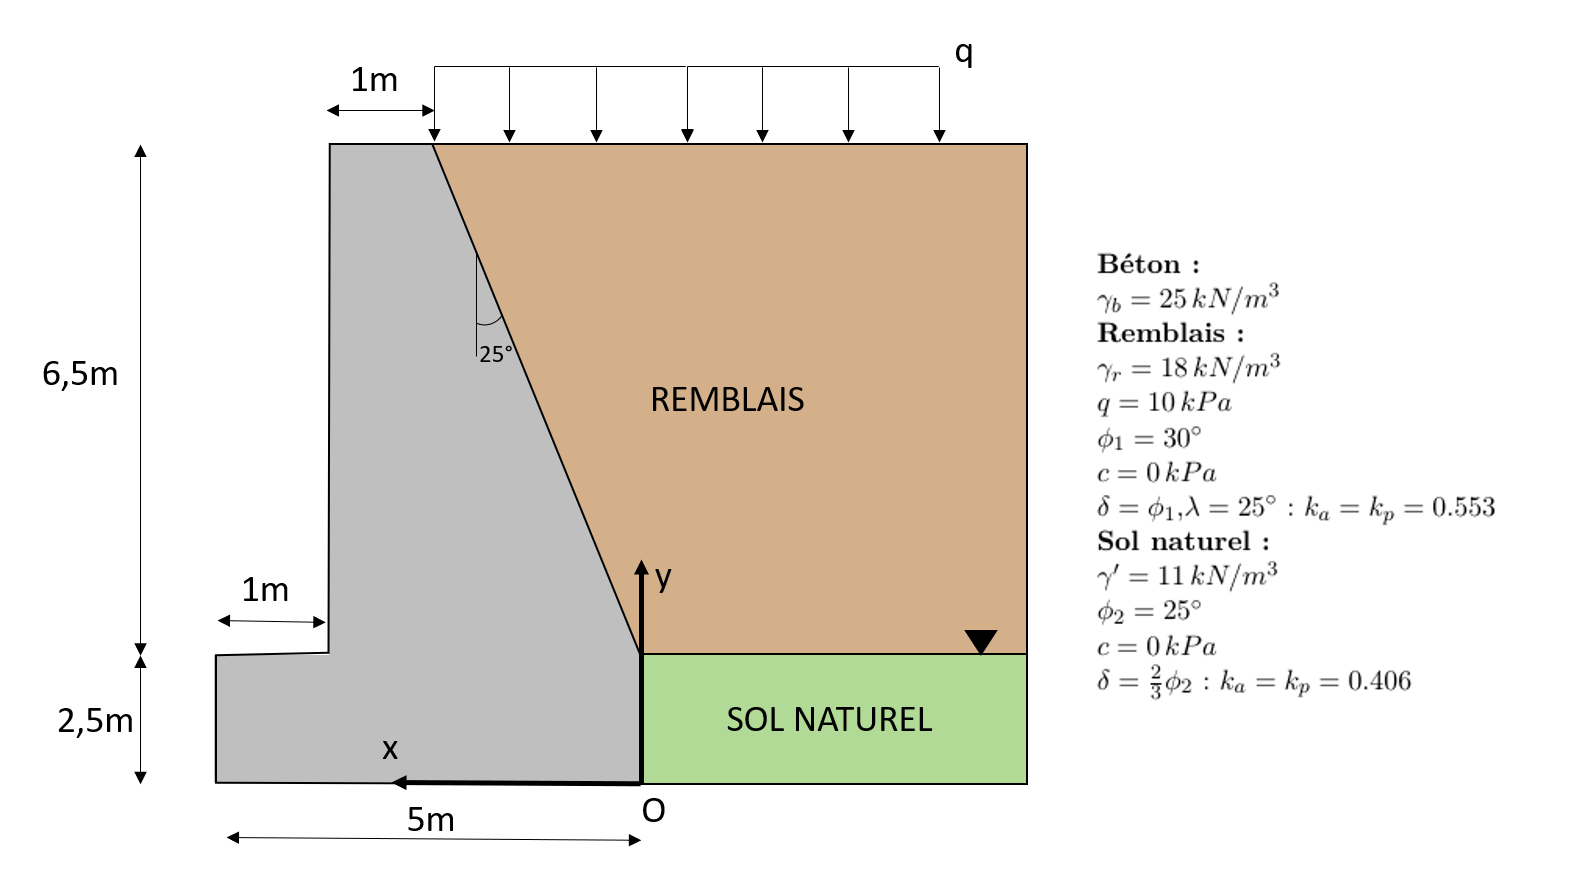
\includegraphics[width=\linewidth]{ex3}
\end{center}

On note que l'angle $\delta$ est mesuré par rapport à la normale à chaque face.


\begin{enumerate}
\item Déterminer pour chacune des grandeurs suivantes leur composantes dans le repère (O,x,y) et leur point d'application:
\begin{itemize}
\item $W$, le poids du mur de soutènement
\item $P_1$, la contrainte du remblais du sur la face inclinée du mur
\item $P_2$, la contrainte du sol naturel sur le bas du mur
\item $Q_1$, la contrainte due à la surcharge q sur la face inclinée du mur
\item $Q_2$, la contrainte due à la surcharge q sur le bas du mur
\end{itemize}
\item  Déterminer l'excentricité $e$ de la résultante $F_v$
\begin{center}
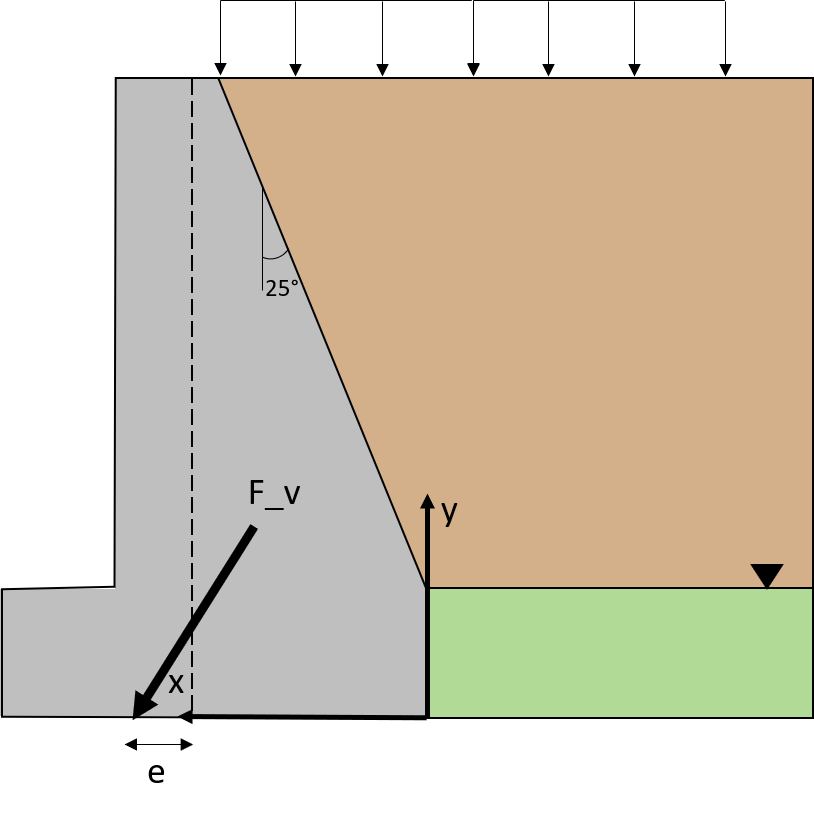
\includegraphics[width=0.4\linewidth]{ex3b}
\end{center}
\item En sachant que 
$$\sigma_{max} = \frac{F_v}{B}(1+\frac{6e}{B})$$
\begin{center}
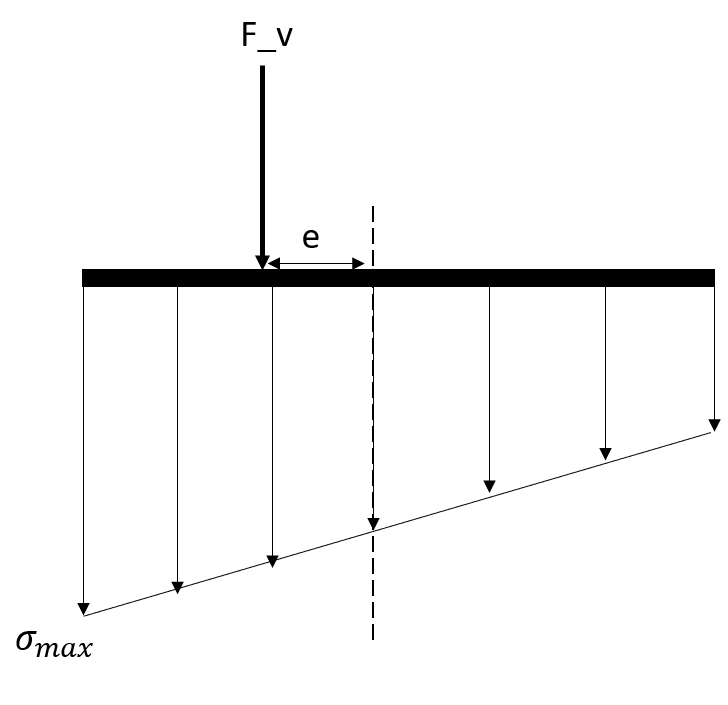
\includegraphics[width=0.4\linewidth]{ex3c}
\end{center}
Calculer la capacité portante selon la formule de Hansen avec les coefficients de Vesic. Déterminer la stabilité au glissement et au renversement par rapport à l'extrémité du mur (en bas à gauche).
\end{enumerate}
%\textbf{Béton :}\\
%$\gamma_b = 25\,kN/m^3$\\
%\textbf{Remblais :}\\
%$\gamma_r = 18\,kN/m^3$\\
%$q=10\,kPa$\\
%$\phi_1 = 30^{\circ}$\\
%$c=0\,kPa$\\
%$\delta =\phi_1$,$\lambda = 25^{\circ}$ : $k_a=k_p=0.553$\\
%\textbf{Sol naturel :}\\
%$\gamma' = 11\,kN/m^3$\\
%$\phi_2 = 25^{\circ}$\\
%$c=0\,kPa$\\
%$\delta =\frac{2}{3}\phi_2$: $k_a=k_p=0.406$


\newpage
\section{Théorie}
Il donnait des grand thèmes et voulait des explications sous formes d'hypothèses, graphes (axes!), schémas, équations.
\subsection{Chapitre Consolidation} Globalement tout le chapitre 1, il donnait des sous questions pour aiguiller.
\begin{itemize}
\item Définir consolidation
\item Essai oeudometrique
\item Courbes oeudometriques et mise en equations
\item Vitesse de consolidation et paramètres qui l'influence 
\item Définir degré de consolidation et contrainte de préconsolidation

\end{itemize}

\subsection{Chapitre Pieux}
Idem, tout le chapitre avec des sous questions pour aiguiller
\begin{itemize}
\item Différencier les fondations superficielles et profondes
\item Donner les différents mode de fonctionnement des pieux
\item Donner la capacité portante d'une fondation profonde
\item Expliquer la méthode classique (charge limite)
\item Expliquer la méthode semi-empirique (charge limite)
\item Pour la méthode semi-empirique, détailler les concepts d'effets d'échelle et méthodes de lissage\footnote{Je sais pas trop jusqu'à quel niveau de détail il voulait qu'on aille...}

\end{itemize}

\subsection{Définitions}
Définir les concepts suivants:
\begin{itemize}
\item Coefficients de poussée des terres actif et passif
\item Contraintes p,q,p' et chemin de contrainte
\item Pôle du cercle de Mohr
\item Indice de frottement (CPT)
\end{itemize}
\end{document}
